\documentclass[oneside,11pt]{fithesis2}  
\usepackage[czech]{babel}
\usepackage[utf8x]{inputenc} 
\usepackage[T1]{fontenc}  
\usepackage[plainpages=false,pdfpagelabels,unicode]{hyperref}  
\usepackage{microtype}
\usepackage{fancyvrb}
\usepackage{url}
\usepackage{hyperref}
\usepackage{graphicx}

\usepackage{cmap}	 % bod b) [do PDF bude přidáván potřebný font resource]
\usepackage[T1]{fontenc} % část bodu a) [vhodné kódování fontů]
\usepackage{lmodern}	 % část bodu a) [vhodný font]
\usepackage{listings}

 
\thesistitle{Relační přístup k Amazon SimpleDB} 
\thesissubtitle{Diplomová práce}  
\thesisstudent{Radim Hopp}    
\thesiswoman{false}          
\thesisfaculty{fi}  
\thesisyear{Podzim 2013}  
\thesisadvisor{Mgr. Marek Grác}  
\thesislang{cs}            

\usepackage[plainpages=false,pdfpagelabels]{hyperref} 
\hyphenation{check-box}
\begin{document}  
\VerbatimFootnotes
\FrontMatter  
\ThesisTitlePage  

\setcounter{page}{1} 

\begin{ThesisDeclaration}  
\DeclarationText  
\AdvisorName  
\end{ThesisDeclaration}   

\begin{ThesisThanks}  
Rád bych poděkoval vedoucímu práce Mgr. Marku Grácovi za ochotný přístup a věnovaný čas, panu Lukáši Tinklovi a lidem z komunity KDE na IRC kanále \#kde-devel za cenné rady.
\end{ThesisThanks}  
 
\begin{ThesisAbstract}  
Cílem této práce bylo důkladné prozkoumání stavu Kiosk Frameworku v KDE 4.x, zjištění stavu nástroje kiosktool v KDE 4.x a doplnění jeho funkčnosti.
\end{ThesisAbstract}  
 
\begin{ThesisKeyWords}  
KDE, Kiosk Framework, kiosktool, Qt
\end{ThesisKeyWords}  
 
\MainMatter

\tableofcontents   
\chapter{Úvod}
Lorem ipsum dolor sit amet, consectetur adipiscing elit. Donec blandit turpis sit amet nibh volutpat ultrices. Quisque ut placerat quam. Nunc pharetra non metus in vestibulum. In in leo porta, rutrum nisi a, scelerisque dolor. Donec non vehicula dui. Ut ut urna quis massa sollicitudin laoreet sed et sapien. Quisque pellentesque massa quam, vitae vulputate enim venenatis id. Curabitur ornare enim leo, et venenatis orci interdum id. Vivamus nunc augue, dictum eu semper consequat, vestibulum vitae eros. Phasellus sodales tincidunt odio, vel rhoncus orci dignissim eu.

Curabitur urna purus, varius id mattis adipiscing, aliquam et sem. Duis sed enim non nisl commodo molestie. Vestibulum gravida suscipit lectus vitae interdum. Maecenas quis vestibulum nibh. Nunc vel porta massa. Sed interdum tortor ac elit sollicitudin, ut auctor nisi ullamcorper. Integer nec eros tempus arcu convallis molestie consectetur ac nunc.

Pellentesque non posuere quam, et ultricies odio. Phasellus varius arcu ac arcu elementum venenatis. Aliquam tempor elit et urna suscipit facilisis. Quisque id ligula nec justo malesuada egestas vel eget nulla. Phasellus non bibendum sem. Ut venenatis quam id nibh cursus, ac convallis metus adipiscing. Integer imperdiet, lorem et ullamcorper pellentesque, ligula mi auctor elit, ut suscipit purus lorem in nibh. Ut aliquam nibh non adipiscing dignissim. Duis consectetur dui ac turpis semper, non lacinia metus feugiat. Aliquam malesuada congue felis eu luctus.

Nam id volutpat metus, vitae sodales enim. Nullam tempor odio libero, id iaculis magna pellentesque accumsan. Vestibulum accumsan mauris quis urna sodales, placerat imperdiet metus tincidunt. Nullam consequat purus sit amet purus consectetur porttitor. Praesent fringilla vitae turpis rutrum rhoncus. Aenean tincidunt, mauris in mattis ornare, dui elit lobortis enim, et elementum libero nulla ut sapien. Class aptent taciti sociosqu ad litora torquent per conubia nostra, per inceptos himenaeos. Suspendisse commodo leo placerat rhoncus adipiscing. Etiam rhoncus rhoncus interdum. Sed sed nibh ut sapien varius sodales. Maecenas lacinia nunc eu neque tempus aliquet.

Vestibulum tempus laoreet lectus. Mauris accumsan velit ac erat condimentum pellentesque. Suspendisse et lorem vitae lorem volutpat interdum. Cum sociis natoque penatibus et magnis dis parturient montes, nascetur ridiculus mus. Sed ac tincidunt leo, sed vulputate mi. Maecenas et nulla egestas, adipiscing neque a, blandit massa. Nam ullamcorper, tortor id accumsan consectetur, tortor neque ultrices mi, a laoreet odio ipsum et tellus. Duis lobortis faucibus luctus.

% Následují další kapitoly a podkapitoly, popřípadě závěr, dodatky, 
% seznam literatury či použitých obrázků nebo tabulek.


\chapter{JBoss Teiid}
JBoss Teiid je otevřený software pro virtualizaci dat z více zdrojů. Tento projekt je zaštiťován v rámci JBoss komunitních projektů\footnote{http://www.jboss.org/overview/} spolu s projekty jako WildFly nebo GateIn\footnote{kompletní seznam projektů na http://www.jboss.org/projects}.

Firma Red Hat nabízí také plně podporovanou a certifikovanou verzi pod názvem Red Hat JBoss Enterprise Data Services Platform. Tento produkt kromě projektu Teiid v sobě obsahuje také JBoss Enterprise Application Platform a další produkty\footnote{kompletní seznam produktů a projektů obsažených v Red Hat JBoss Enterprise Data Services Platform i s použitými verzemi k naleznutí na https://access.redhat.com/site/articles/112333}

\section{Části JBoss Teiid}
\begin{itemize}
 \item \textbf{Query engine}
 
 Jedná se o srdce projektu, které zpracovává relační, XML, XQuery a jiné dotazy ze zdrojů dat. Také zajišťuje podporu pro schémata vytvořené z jednoho, či z více různých zdrojů dat. V neposlední řadě se query engine stará o transakce a uživatelem definované funkce.
 
 \item \textbf{JDBC ovladač}
 
 JDBC ovladač slouží pro jednoduché použití Teiidu v ostatních java aplikacích.
 
 \item \textbf{Server}
 
 Tato část je zodpovědná za běh query enginu v rámci aplikačního serveru (WildFly nebo Red Hat JBoss Enterprise Application Platform) a zaručuje škálovatelnost a snadnou správu. Součástí je administrační konzole, ve které je možno jednoduše nastavit například deploynutou virtuální databázi nebo nastavení vláken query enginu.
 
 \item \textbf{Konektory a překladače}
 
 Teiid přichází s řadou konektorů a překladačů, díky kterým je schopen napojit se na řadu různých zdrojů dat. Konektory zajišťují napojení na zdroj dat, překladače potom obstarávají získávání dat podle Teiid požadavků. Základním kamenem jsou konektory pro většinu relačních databází, webové služby, textových souborů a LDAP\footnote{Lightweight Directory Access Protocol)}.
 
 Cíl této diplomové práce je rozšířit tuto sekci o connector pro NoSQL databázi Amazon SimpleDB.
 
 \item \textbf{Nástroje}
 
  \begin{itemize}
  \item Teiid Designer
  
  Teiid Designer je separátní projekt (není součástí projektu JBoss Teiid), který ovšem také patří mezi komunitní projekty jboss.org. Jedná se o sadu zásuvných modulů pro vývojové prostředí Eclipse, které usnadní definování virtuálních databází (pohledy, procedury, ...)
  
  \item Nástroje pro monitorování a správu
  
  Dvěmi hlavními nástroji pro monitorování a správu jsou Teiid Web Console (V zásadě jde o rozšíření webové konzole aplikačního serveru o položky pro správu a monitorování Teiid instance) a zásuvný modul pro RHQ\footnote{RQH je komunitní projekt vedený pod jboss.org pro správu více serverů, http://www.jboss.org/rhq} pro kontrolu více serverů či clusterů Teiidu.
  
  \item Skriptování
  
  V rámci Teiidu je také distribuován Teiid AdminShell, což je skriptovací nástroj založený na jazyku Groovy. AdminShell umožňuje spravovat Teiid z příkazové řádky či pomocí skriptu, což uživateli velmi usnadní provádění často se opakujících činností.
  
  \end{itemize}

\end{itemize}

\chapter{Amazon SimpleDB}
SimpleDB je databáze z dílen firmy Amazon a patří do skupiny produktů Amazon Web Services. Tato databáze je takzvaná NoSQL, což znamená, že data v ní jsou uložená ve formátu, jaký není běžný pro relační databáze (tabulky, sloupce, řádky). SimpleDB je poskytována firmou Amazon jako služba. To znamená, že není možné nasadit si databázi SimpleDB na vlastním serveru, ale běží pouze na serverech firmy Amazon. 
\section{Struktura databáze SimpleDB}
Struktura SimpleDB databází je možno přirovnat k tabulkovému procesoru.
\begin{itemize}
 \item \textbf{Uživatelský účet (Customer Account)}
 
 V rámci jednoho účtu lze mít více domén stejně jako v rámci jednoho souboru tabulkového procesoru je možno mít více listů s tabulkami.
 \item \textbf{Doména (Domain)}
 
 Analogie k jedné tabulce v tabulkovém procesoru. Obsahuje řádky (položky), sloupce (atributy) a jednotlivé buňky (hodnoty).
 \item \textbf{Položky (Items)}
 
 Řádky tabulky. Reprezentují jednotlivé objekty uložené v databázi s jedním, či více vyplněnými atributy.
 \item \textbf{Atributy (Attributes)}
 
 Sloupce tabulky. Určují kategorie dat, jakých můžou položky nabývat.
 
 \item \textbf{Hodnoty (Values)}
 
 Hodnoty si lze představit jako jednotlivé buňky tabulky. Tady se ovšem analogie s tabulkovým procesorem rozchází, neboť jedna \uv{buňka} může nabývat více hodnot najednou.
 
\end{itemize}
Navíc má každý prvek domény (řádek tabulky) povinný atribut \verb<ItemName<, který musí být v dané doméně unikátní.

SimpleDB nepoužívá žádné jiné datové typy krome typu \verb<String<, takže i čísla jsou v databázi uloženy a je s nimi nakládáno jako s textovými řetězci. To s sebou nese řadu problémů a hlavně zátěž na vývojáře aplikace tyto problémy řešit. Typickým příkladem takového problému je, že čísla nejdou řadit lexikograficky ( lexikograficky: 10<2, což je špatně). Řešením je doplnění nul před čísla (00010>00002, což je správně).

\section{Vlastnosti databáze Amazon SimpleDB}
\subsection*{SimpleDB jako služba}
Databáze Amazon SimpleDB je dodávaná jako služba. To znamená, že Amazon neposkytuje možnost nasadit tuto databázi ve vlastním prostředí, ale provozuje ji pouze na svých serverech. Uživatel databáze se tedy nemusí starat o nastavování ani o hardware, ale například ani o škálování, nebo o replikaci dat, jelikož Amazon automaticky distribuuje a synchronizuje data v několika datových centrech umístěných v různých geografických zónách, čímž omezuje nejen riziko ztráty dat, ale také zvyšuje rychlost přístupu k datům v různých místech na světě. Tím pádem se může uživatel databáze plně zaměřit na práci s vlastními daty.
\subsection*{Flexibilita}
Flexibilita je další výhoda databáze Amazon SimpleDB. Jelikož je to NoSQL databáze není potřeba mít pevně dané schéma, jak tomu bývá u SQL databází, ale nové atributy a entity mohou být přidávány takzvaně za pochodu.
\subsection*{Indexování}
SimpleDB automaticky indexuje veškeré data v ní uložené, čímž tato povinnost odpadá z beder vývojářů aplikace a zvyšuje rychlost navracení výsledků čtecích operací.	
\subsection*{Konzistence}
Amazon pro zápis zaručuje konzistenci takovou, že úspěšně provedený zápis (použitím příkazů jako např. \emph{PutAttributes}, \emph{BatchPutAttributes}, \emph{CreateDomain}, \dots) znamená, že všechny kopie databáze byly změněny. Toto pojetí konzistence ovšem nezaručuje chování při překrytí dvou či více zápisů najednou. Pouze zaručuje, že výsledné data budou na všech kopiích databáze rovná hodnotě jednoho z těchto zápisů (toho, který databáze obdržela nejpozději). toto bude níže ilustrováno na příkladě.
Při čtení si uživatel může zvolit mezi konzistentním a eventuálně konzistentním čtením. Konzistentní čtení zaručuje, že vrátí hodnotu po provedení posledního dosud přijatého zápisu. Eventuálně konzistentní čtení na druhou stranu vrátí hodnotu, která je aktuálně uloená na dotazovaném serveru (tj. může vrátit již neplatnou hodnotu).
\subsubsection*{Příklad konzistence}
Na obrázku 3.1 je uveden příklad, kdy se překrývají dva zápisy. V této situaci není možné určit, jestli pro provedení obou zápisů bude výsledná hodnota atributu \verb<Barva< rovna \verb<červená<, nebo \verb<zelená< z toho důvodu, že není zaručeno, kterou instrukci zpracuje SimpleDB jako první. Například kvůli vysoké latenci sítě prvního klienta bude nejprve přijata a zpracována instrukce \verb<W2< druhého klienta a následně přepsána instrukcí \verb<W1<, tedy veškeré následné konzistentní čtení vrátí \verb<Barva=červená<.

Jak bylo ukázáno, konzistentní čtení v tomto případě mohlo vrátit jak výsledek \verb<W1<, tak výsledek \verb<W2<. Oproti tomu, výsledek eventuálně konzitentního čtení může být kromě \verb<W1< či \verb<W2< také \verb<nic<. Pravděpodobnost prázdného výsledku se s časem minimalizuje, neboli čím déle po zápisu je čteno, tím větší je pravděpodobnost korektního výsledku.
\begin{figure}[h]
 \caption{Ilustrace chování databáze SimpleDB}
 \centering
 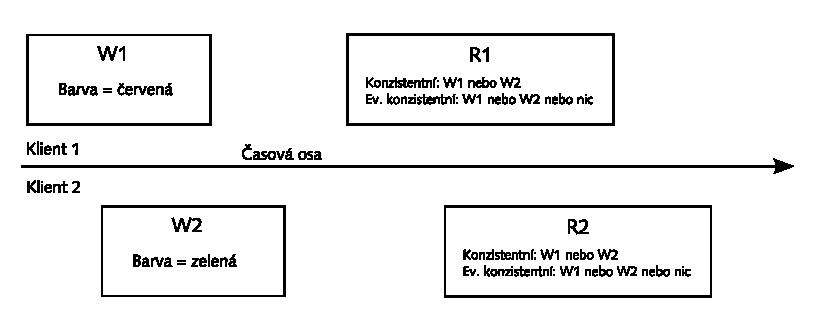
\includegraphics[scale=0.9]{ConsistencyExample}
\end{figure}
%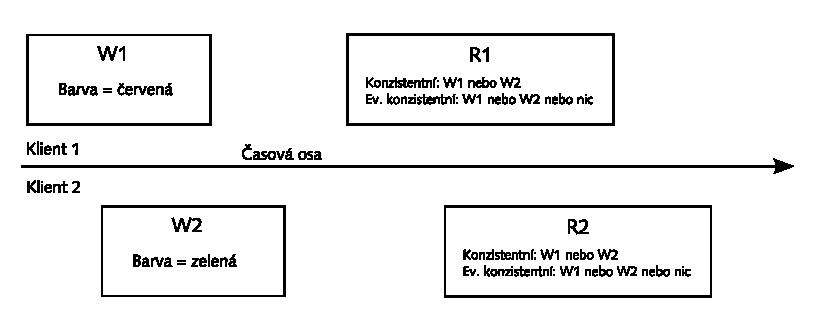
\includegraphics{ConsistencyExample}

Základní rozdíl mezi konzistentním a eventuálně konzistentním čtením lze shrnout do tabulky:
\begin{figure}[h]
 \caption{Tabulka vlastností konzistentního a ev. konzistentního čtení}
 \vspace{5mm}
 \begin{tabular}{l|l}
    Eventuálně konzistentní čtení & Konzistentní čtení\\ \hline
    Možné nekorektní výsledky & Vždy korektní výsledek\\ 
    Rychlejší odezva & Možná pomalejší odezva \\
    Větší dataová propustnost & Možná menší datová prostupnost
 \end{tabular}
\end{figure}

\subsection*{Omezení databáze SimpleDB}
Kromě výše zmíněného chování, které by se v jistých situacích dalo považovat za omezení, je asi největším omezením velikost domény, jak co se místa na disku týče, tak také maximální počet atributů. Konkrétně je horní hranice 10 GB pro data a 1 miliarda atributů na jednu doménu. Domén je možno vytvořit až 250 na jeden uživatelský účet.


\chapter{Komunikace s databází Amazon SimpleDB}
\subsection*{Přehled příkazů SimpleDB}
\begin{itemize}
 \item \textbf{CreateDomain} slouží k vytvoření nové domény.
 \item \textbf{DeleteDomain} vymaže danou doménu.
 \item \textbf{ListDomains} vrátí seznam domén asociovaných s daným uživatelským účtem.
 \item \textbf{DomainMetadata} slouží k získání informací o dané doméně (datum vytvoření, počet položek v doméně, počet atributů, \dots)
 \item \textbf{PutAttributes} vloží novou položku s danými hotnotami atributů, či upraví již stávající položku.
 \item \textbf{Select} se podobá běžnému \verb<SELECT< příkazu, který je dobře známý z SQL jazyků. Je ovšem mírně omezen a to například absencí \verb<JOIN< klauzule. Přesný přehled možností příkazu \verb<SELECT< databáze SimpleDB je uveden v dokumentaci\footnote{http://awsdocs.s3.amazonaws.com/SDB/latest/sdb-dg.pdf}
 \item \textbf{GetAttributes} vrátí hodnoty požadovaných atributů jedné dané položky. Umožňuje specifikovat jeden, či více požadovaných atributů, nebo také všechny atributy dané položky.
\end{itemize}

\subsection*{Podmíněné vkládání a mazání dat}
SimpleDB v aktuální verzi (od 24. února 2010) podporuje takzvaný podmíněný zápis a mazání dat. 

Při tomto podmíněném zápise (mazání) se spolu s běžnými parametry odešle také podmínka a očekávaný výsledek vyhodnocení dané podmínky. Zápis se poté provede pouze tehdy, je-li vyhodnocená podmínka rovna očekávanému výsledku.

Tato vlastnost se dá použít například pro implementaci čítače (přečte aktuální stav čítače a pokusí se zapsat nový stav čítače za podmínky, že stav čítače byl nezměněn), což by bez podmíněného vložení byl netriviální úkol. Také se tímto rozšiřují možnosti kontroly konkurenčního přístupu k datům (pomocí optimistických protokolů).

\subsection*{Bezpečnost}
Pro autentizaci má každý uživatel \uv{ID přístupového klíče} (20 alfanumerických znaků) a \uv{tajný přístupový klíč} (40 alfanumerických znaků), kterými podepisuje kažý požadavek vůči SimpleDB. Sama Amazon SimpleDB nemá nástroj pro autorizaci, ten je ovšem integrován do správy identit a přístupu AWS (AWS Identity and Access Management - systém pro správu uživatelů a jejich práv v rámci celého AWS), takže je možné omezit práva jednotlivým uživatelům. Jediným problémem může být skutečnost, že nelze definovat přístupové práva pro jiný AWS účet -- pro každého uživatele domény musí být vytvořen uživatel v rámci AWS účtu vlastnícího doménu.

\subsubsection*{Proces autentizace}
\begin{enumerate}
 \item Vytvoření řetězce dotazu
 \item Kanonizování řetězce dotazu (seřazení parametrů, zakódování parametrů a jejich hodnot URL kódováním\footnote{Podle RFC 3986, kapitola 2 -- http://tools.ietf.org/html/rfc3986}), \dots)
 \item Vypočítání HMAC\footnote{Podle RFC 2104 -- http://www.ietf.org/rfc/rfc2104.txt} z kanonizovaného textového řetězce za použití \uv{tajného přístupového klíče} jako klíče a SHA256 nebo SHA1 jako hashovacího algoritmu.
 \ Tento podpis se připojí k původnímu požadavku jako parametr \verb<signature< spolu s ID přístupového klíče jako \verb<AWSAccessKeyId<.
\end{enumerate}
Zde je ukázán proces autentizace pouze zjednodušeně. Přesný návod jak sestrojit validná požadavek je dostupný v dokumentaci SimpleDB.

\subsection*{Knihovny pro komunikaci}
Amazon poskytuje knihovny pro komunikaci se SimpleDB (a ostatními AWS službami) v několika jazycích (Java, PHP, Python, Ruby a .NET). 
Knihovna pro jazyk Java, která byla v této práci použita, nejenže poskytuje model pro práci s doménami, atributy a podobně, ale také významně usnadňuje autentizační proces (není nutné \uv{ručně} počítat podpis).
\chapter{Mapování Teiid dotazů na SimpleDB dotazy}
V této kapitole bude obecně ukázáno, jakým způsobem byly mapovány Teiid dotazy na dotazy databáze SimpleDB. Konkrétně se jedná o příkazy \verb<SELECT<, \verb<INSERT<, \verb<UPDATE< a \verb<DELETE<.
\section{Vícehodnotové atributy}
Teiid přistupuje k datům jako běžná relační databáze, tedy jednomu řádku a sloupci odpovídá nejvýše jedna hodnota. Z tohoto důvodu je nutné ošetřit přístup k vícehodnotovým atributům. Nabízí se několik řešení:
\begin{enumerate}
 \item Byl-li by dopředu znám maximální počet hodnot u jednotlivých atributů, mohl by Teiid vnímat vícehodnotové atributy jako více sloupců tabulky (pro každou z možných hodnot jeden sloupec). Tímto přístupem by se ovšem zafixovalo schéma a přišli bychom o jednu z hlavních výhod databáze SimpleDB (SimpleDB netrvá na pevném schématu).
 \item Zakódovat všechny hodnoty vícehodnotového atributu do jediného textového řetězce, který by byl lidsky i strojově čitelný. Tímto odpadá problém se změnou počtu hodnot atributu.
\end{enumerate}
Ve finální implementaci byl zvolen druhý přístup a hlouběji bude probrán níže.

\section{SELECT}
Jelikož SimpleDB podporuje mírně omezený \verb|SELECT|, stačí vždy pouze poupravit řetězec příkazu \verb|SELECT| generovaný Teiidem, aby byl srozumitelný pro SimpleDB. Naštěstí lze pro každý překladač nadefinovat sadu podporovaných vlastností. Nepodporované vlastnosti obslouží sám Query Engine (např. překladač nepodporuje \verb<JOIN< klauzuli. Query Engine tedy rozloží dotaz s \verb<JOIN< klauzulí na dva jednoduché dotazy, ty poté předá překladači a výsledné data zpracuje programově v paměti).

Struktura příkazu SELECT databáze SimpleDB:
\begin{Verbatim}[frame=leftline,fontsize=\small]
select output_list
from domain_name
where [expression]
[sort_instructions]
limit [limit] 
\end{Verbatim}
Ze struktury je zřejmé, že žádné velké změny nebude třeba provádět. Je nutné definovat, že překladač nepodporuje \verb<JOIN< klauzuli a poté zajistit, aby byly korektně prováděny jednoduché SQL dotazy na které byl původní dotaz rozložen. Zde vyvstává pár problémů:
\begin{enumerate}
 \item Dotazu obsahujícímu atribut \verb<itemName()< (povinný unikátní atribut, který má každá položka) musí být tento atribut odebrán -- tento atribut je automaticky vracen v odpovědi databáze ikdyž není specifikován. Naopak pokud je požadován spolu s jinými atributy, databáze vrátí chybu. Toto platí s výjimkou dotazu, kdy je \verb<itemName()< jediným požadovaným atributem.
 
 Tento dotaz je korektním dotazem na databázi SimpleDB a vrátí hodnoty atributu \verb<itemName()< všech položek v doméně \verb<TestDomain<:
 \begin{Verbatim}[fontsize=\small]
SELECT itemName() FROM TestDomain
  \end{Verbatim}
 Tento dotaz vrátí chybovou hlášku \verb<InvalidQueryExpression<:
  \begin{Verbatim}[fontsize=\small]
SELECT itemName(), attribute1 FROM TestDomain
  \end{Verbatim}
 \item Další problém může vyvstat ve výrazu ve \verb<WHERE< části. Těmto potížím se dá vyhnnout správným nastavením schopností překladače. 
\end{enumerate}

\section{INSERT}
Zde je situace stále celkem jednoduchá, neboť \verb<INSERT< vždy vkládá jeden nový řádek, což je téměř ekvivalentní příkazu \verb<PutAttributes<. Je zde akorát potřeba získat z Teiid příkazu \verb<INSERT< seznam sloupců, jejich hodnot a název domény do které má proběhnout vložení. Vzhledem ke zvolenému řešení problému vícehodnotových atributů není zde nutné se jimi zaobírat.
\section{UPDATE}
U \verb<UPDATE< je situace poněkud složitější, neboť je možné měnit více položek najednou (díky \verb<WHERE< klauzuli) a příkazy \verb<PutAttributes< a \verb<BatchPutAttributes< neumožňují měnit více položek specifikovaných pomocí kritéria najednou. Je tedy nutné nejprve pomocí \verb<SELECT< příkazu nad požadovanou doménou a kritérii z Teiid \verb<UPDATE< dotazu získat jména všech upravovaných položek (atribut \verb<itemName()<). Teprve poté lze pomocí několika \verb<PutAttributes<, či jediného \verb<BatchPutAttributes< dané položky upravit.
\section{DELETE}
Podobně jako u příkazu \verb<UPDATE< je nejprve potřeba získat jména všech položek, které mají být smazány a ty následně pomocí \verb<DeleteAttributes< smazat z databáze.
\chapter{Implementace}
V této kapitole bude rozebrána konkrétní implementace, problémy, které se během implementace vyskytly, a jejich řešení.
\section{Konektor}
Základním kamenem a prvním krokem v implementaci bylo vytvoření konektoru.

Java EE Connector Architecture (JCA) je standardizované řešení pro připojení k podnikovým informačním systémům (enterprise information systems). Stejně jako je JDBC zodpovědné pro připojení Java EE aplikací k databázím, JCA je obecnější architektura pro připojení k systémům, pro které není vytvořen JDBC ovladač. Základem každého konektoru je tzv. resource adapter, jež je odpovědný za přístup a interakci s daným informačním systémem, který cheme řipojit. Jednotlivé Java EE aplikace, nasazené v aplikačním serveru, poté tento resource adapter využívají pro komunikaci. 

Specifikace JCA je vyvíjena v rámci Java Community Process jako JSR 322\footnote{Dostupné na webu Java Community Process -- http://www.jcp.org}
\subsection*{Modul simpledb-api}
Tento modul reprezentuje API pro komunikaci s databází simpledb a jako samostatný modul vzniknul hlavně kvůli oddělení závislostí na java knihovnu pro komunikaci se SimpleDB (aws-java-sdk) od ostatních modulů.

Tento modul obsahuje pouze jednu java třídu a jedno rozhraní a to \verb<SimpleDBAPIClass< a \verb<SimpleDBConnection<.
\begin{itemize}
 \item \verb<SimpleDBConnection< je rozhraní rozšiřující rozhraní \verb<Connection< z balíčku \verb<javax.resource.cci< (\verb<Connection< reprezentuje připojení na extern zdroj na aplikační vrstvě -- díky třídám implementující toto rozhraní je možné přistupovat k požadovaným zdrojům).
 \item \verb<SimpleDBAPIClass< je třída zaobalující potřebné příkazy databáze SimpleDB. Za povšimnutí stojí hlavně metoda \texttt{Set<String> \\* getAttributeNames(String domainName)}, která vrací jména všech atributů v doméně, ovšem jediný způsob jak toho docílit je provedení příkazu \texttt{SELECT * FROM <domainName>} a z odpovědi získat jména všech atributů (nestačí dotázat se například na jednu položku, neboť kdyby daná položka neměla vyplněný nějaký atribut, tento atribut by v odpovědi nebyl obsažen).
\end{itemize}
\subsection*{Modul connector-simpledb}
Jedná se o plnohodnotný, ikdyž poměrně jednoduchý, Java EE konektor pro SimpleDB. Konektory jsou běžně baleny jako RAR (Resource Adapter Archive), které lze poté nasadit na aplikační server pouhým nakopírováním do složky \texttt{deploy} serveru. Teiid poskytuje základní implementaci rozhraní potřebných pro vytvoření zákadního konektoru. Zde bylo důležité uzpůsobit tuto základní implementaci potřebám databáze SimpleDB. 
\begin{itemize}
 \item Třída \texttt{SimpleDBManagedConnectionFactory} rozšiřuje abstraktní třídu \texttt{BasicManagedConnectionFactory} (základní Teiid implementace). V této třídě je nutno definovat proměnné, které jsou potřebné pro připojení ke zdroji -- tedy proměnné ve kterých bude uložen ID přístupového klíče a tajný přístupový klíč spolu s metodami pro jejich nastavení a získání (get a set metody). Požadované hodnoty budou aplikačním serverem získány z konfiguračního souboru serveru (typicky třeba \texttt{standalone.xml}) a injectovány do těchto proměnných. Další důležitou částí je implementace abstraktní metody \texttt{creteConnectionFactory()}, pomocí které je vytvořena instance \texttt{ConnectionFactory}. Ta slouží k generování jednotlivých připojení ke zdroji dat (SimpleDB).
 \item Jako implementace rozhraní \texttt{Connection} zde slouží třída \texttt{SimpleDB ConnectionImpl}. Ta kromě implementování rozhraní \texttt{Connection} rozšiřuje základní Teiid implementaci \texttt{BasicConnection}. Nám zde tedy stačí zajistit přístup k instanci třídy \texttt{SimpleDBAPIClass}. To je splněno instanciováním v konstruktoru a přiřazením do privátní proměnné, která je poté dostupná pomocí její get metody.
 
 S takto připraveným připojením lze poté v samotném překladači snadno volat metody definované v \texttt{SimpleDBAPIClass} např. takto:
 \begin{Verbatim}[fontsize=\small]
((SimpleDBConnectionImpl)connection).getAPIClass().getDomains();
 \end{Verbatim}
 \item Dalším krokem je vytvoření konfiguračních souborů \texttt{MANIFEST.MF} a \texttt{ra.xml}. Oba soubory je nutno umístit do složky \texttt{META-INF}. 
 
 \texttt{MANIFEST.MF} obsahuje pouze závislosti resource adapteru. V případě našeho konkrétního adapteru je to:
 \begin{Verbatim}[fontsize=\small]
Dependencies: org.jboss.teiid.common-core,org.jboss.teiid.api,
	    javax.api,org.jboss.teiid.translator.simpledb.api
 \end{Verbatim}
 
 V deployment descriptoru \texttt{ra.xml} definujeme hlavní třídu resource adapteru (tj. třída implementující rozhraní \texttt{Resource Adapter}), třídu implementující rozhraní \texttt{ManagedConnectionFactory} a definujeme proměnné potřebné k připojení k SimpleDB (ID přístupového klíče a tajný klíč). 
 
 \item Celý tento modul je poté běžně zkompilován a balen jako Resource Adapter Archive -- RAR (běžný Java archive -- JAR s příponou \texttt{.rar}), který může být nasazen na aplikační server zkopírováním do složky \texttt{deploy/}. 

\end{itemize}


\chapter{Tutoriál}
\chapter{Závěr}
\bibliographystyle{plain}  % bibliografický styl 
\bibliography{mujbisoubor} % soubor s citovanými
                           % položkami bibliografie 

\end{document}
